\chapter{Laparoscope Testing}
\label{sec:test}


In this chapter of the report, all the documentation of the tests performed for this skripsie can be found. The tests performed can be divided into three sections: validation test; specification test; and functionality test. 

\section{Validation Tests}

The validation tests are tests to determine whether a calculated theoretical value is accurate or not. Currently, there are four validation tests that need to be performed. These tests consist of:

\begin{itemize}
    \item Field of view validation test
    \item Viewing angle validation test
    \item Produced illuminance validation test
    \item Heat transfer model validation test
\end{itemize}

The first two tests are tests created by the International Organization for Standardization to determine the field of view and viewing angle of the laparoscope. ISO~8600-3 describes the test procedures. Additionally, the standard gives the allowable deviation from the theoretical values. For the field of view, the value cannot deviate more than 15~\%, and for the viewing angle, it cannot deviate more than 10°. Table \ref{tab:ISO Tests} below shows the results of these tests:

\begin{table}[h]
    \centering
    \caption{ISO standard test results}
    \begin{tabular}{|c|c|c|c|}

    \hline
        Test & Theoretical Value & Actual Value & Deviation \\
    \hline
        Field of view & 90° & T.B.D. & T.B.D \\
    \hline
        Viewing angle & 30° & T.B.D. & T.B.D \\
    \hline

    \end{tabular}
    \label{tab:ISO Tests}
\end{table}

The third test is to determine how much illuminance is produced by the light source and whether the value is within the expected range. This value is within a range due to the nature of the selected components for the light source. Four White SMD 1206 LEDs were selected to create the light source, and according to their datasheet, they have a luminous intensity value between 200~mcd and 850~mcd and a viewing angle of 120°. The equations below show how the theoretical illuminance can be calculated: \citep{TLH}

\begin{subequations}
    \centering
    \begin{gather}
        \Omega = 2*pi*(1-cos(\Theta/2)) \\
        \Phi = I*\Omega \\
        r = d*tan(\Theta/2) \\
        A = pi*r^2 \\
        E =  \Phi/A 
    \end{gather}
    
\end{subequations}

Here is the list of all the variables used in the equations above:

\begin{itemize}
    \item $\Omega$: Beam solid angle (sr)
    \item $\Theta$: Viewing angle of LED (°)
    \item $\Phi$: Luminous flux (lm)
    \item r: Radius of the illuminated area (m)
    \item d: Distance between the light source and the illuminated area (m)
    \item A: Area of the illuminated area ($m^2$)
    \item E: Illuminance (LUX)
\end{itemize}

Based on the equation above, Table \ref{tab:Illumance Values} below are the expected ranges for the developed product and the measured values for the test:

\begin{table}[h]
    \centering
    \caption{Measured illuminance valued versus expected values}
    \begin{tabular}{|c|c|c|c|}

    \hline
        Distance & Minimum value & Maximum value & Measured value \\
    \hline
        5 & 1 334 LUX & 5 669 LUX & T.B.D \\
    \hline
        100 & 6.66 LUX & 28.32 LUX & T.B.D \\
    \hline

    \end{tabular}
    \label{tab:Illumance Values}
\end{table}

An Illuminance meter will be utilized to measure the illuminance of the laparoscope's light source.

The final test is to validate the heat transfer model, developed in chapter \ref{sec:Heat}. To perform this test, the built product will be turned on for a long duration of time (8~hours), and the temperature in the laparoscope at points of interest will be measured using the built-in sensors. The measured values will be compared to expected values to determine the accuracy of the heat transfer model.

\section{Specification Tests}
Specification tests are required to determine the values and relationships of interest of the laparoscope. For the laparoscope, there are two tests that fall into this category: the heat dissipation test of the camera module and light source, and the digital thermocouples' calibration tests.

The developed product makes use of two digital thermocouples to measure the temperature inside the laparoscope. These thermocouples will be placed in the tip and handle of the product. However, before these components can be placed inside the laparoscope, they need to be calibrated to give the correct measurements. Therefore, the following test was executed.

The digital thermocouples and a calibrated thermocouple were placed within water that was either heated or frozen. In five-minute intervals, the temperature of the water was measured through all the available sensors, until within 5~°C of room temperature. The measured data were then plotted, and the best linear fits were found for each group of data points. Figures \ref{fig:S1-1} and \ref{fig:S1-2} below show the digital sensors' measurements against the calibrated sensor measurements:

\begin{figure}[H]
    \centering
    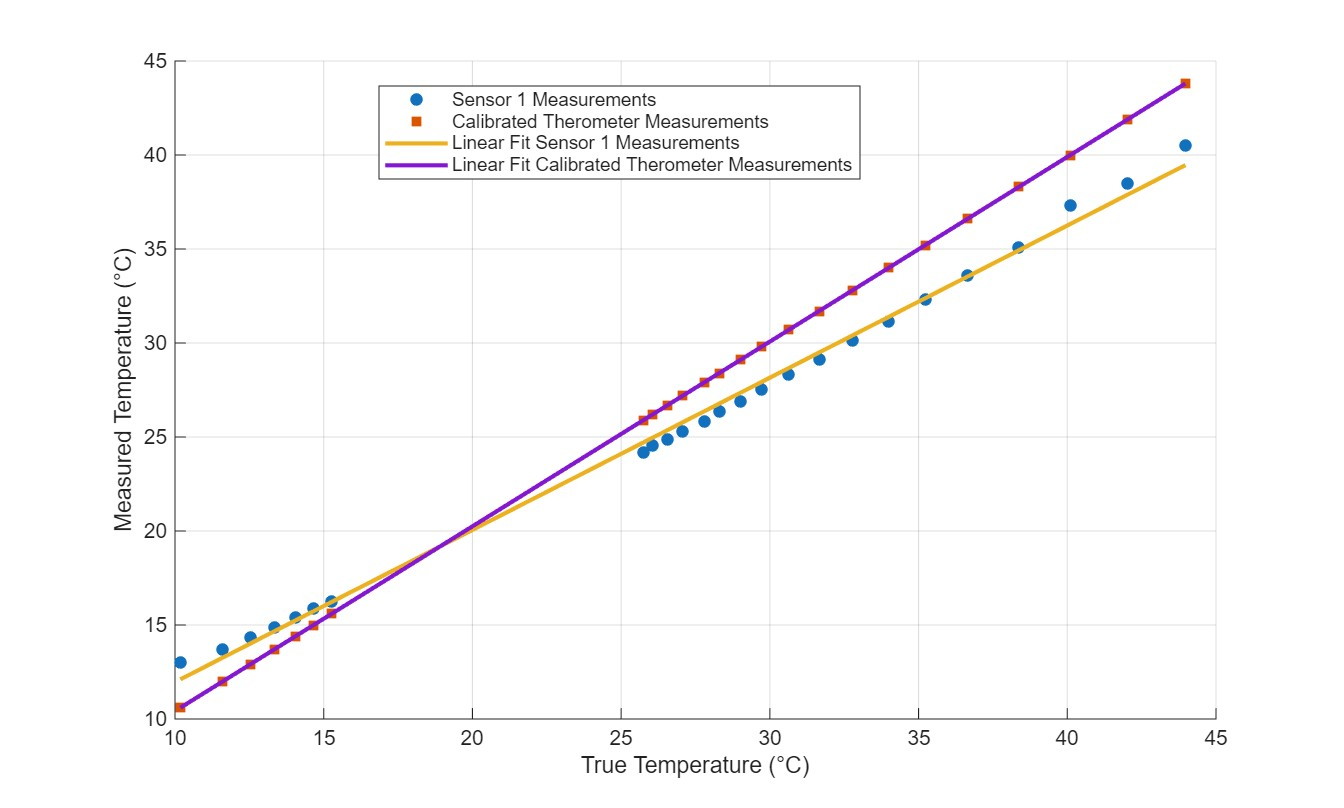
\includegraphics[width=\textwidth]{figs/S1.jpg}
    \caption{Sensor one vs calibrated sensor}
    \label{fig:S1-1}
\end{figure}

\begin{figure}[H]
    \centering
    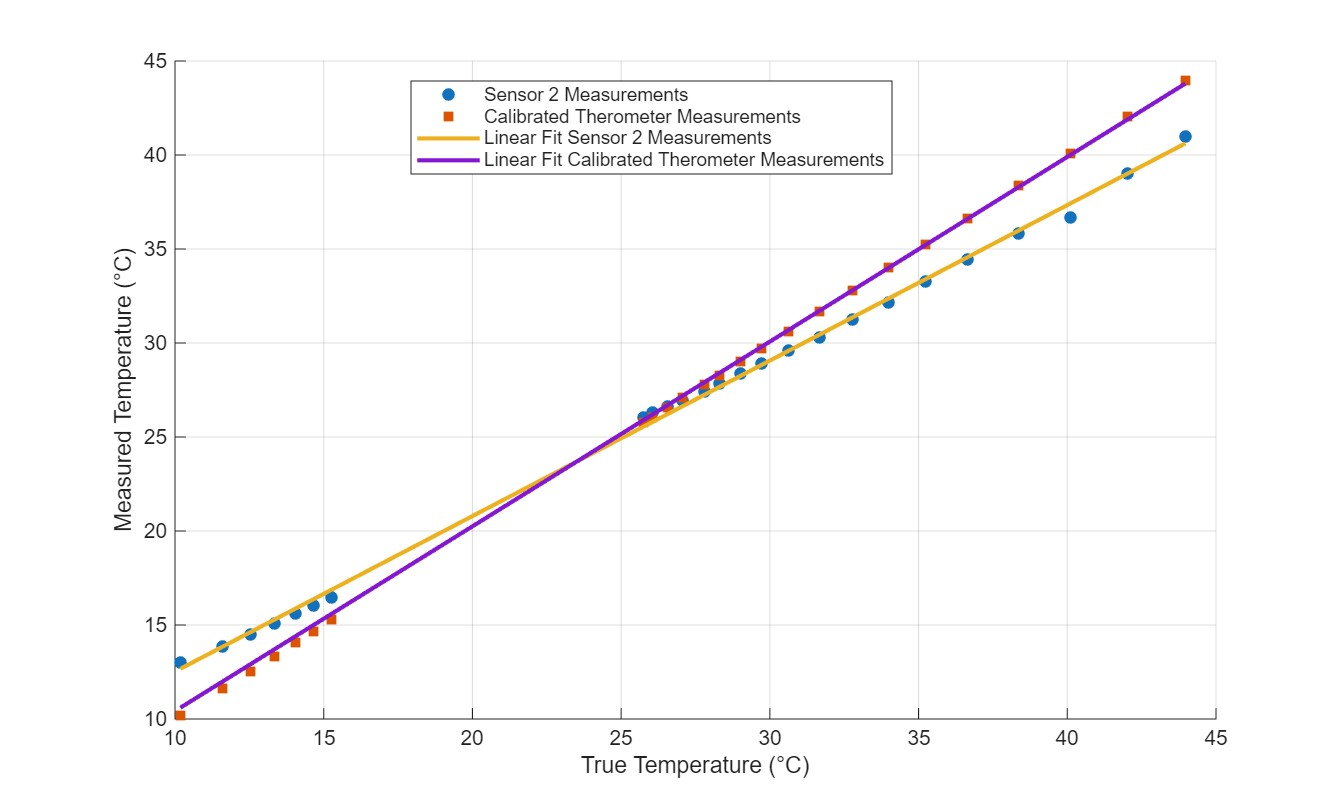
\includegraphics[width=\textwidth]{figs/S2.jpg}
    \caption{Sensor two vs calibrated sensor}
    \label{fig:S1-2}
\end{figure}


Based on the information extracted from the graphs shown above, it appears that the sensor readings have a linear relationship with the true temperature measurements. Therefore, the measured temperatures can be easily converted into the true temperature with the help of the following equations:

\begin{subequations}
    \centering
    \begin{gather}
        Measurement_1 = (Sensor_1(Reading)-3.8676)/0.8095 \\
        Measurement_2 = (Sensor_2(Reading)-4.2511)/0.8271 
    \end{gather}
    
\end{subequations}

The equations mentioned above are derived using the linear polyfit function from Mathworks MATLAB.

The second specification test required for the laparoscope is to determine how much heat is dissipated by the laparoscope’s camera module and light source. This value is important because it will determine whether the design of the laparoscope will be able to dissipate the generated heat effectively or not. It is also critical for the heat transfer model.

To determine how much heat is generated, the camera module and the light source are placed inside a thermal container, with a temperature sensor. The container is then sealed, while the module and light source are turned on. Over two hours, the temperature is periodically measured every ten minutes. The captured data is then processed, and the following information was extracted:

\begin{itemize}
    \item Average heat dissipated = 0.32606 $\mu$W 
    \item Maximum heat dissipated = 3.8865 $\mu$W  
    \item Minimum heat dissipated = - 2.0298 $\mu$W  
\end{itemize}

However, looking at the information extracted from the test, it shows unexpected data. Especially, the minimum heat dissipated value is negative. This means for a period of time, the container got colder instead of hotter. This could be due to inaccuracies of the sensors, because they are only accurate with a 0.5 °C tolerance. However, looking at the Figure \ref{fig:Temperature} below, it shows that it is not just a sensor issue. The most likely explanation for this result is that the container was not properly sealed, which led to heat escaping the container, as well as letting cold air enter the container. Therefore, the experiment will need to be performed again.


\begin{figure}[H]
    \centering
    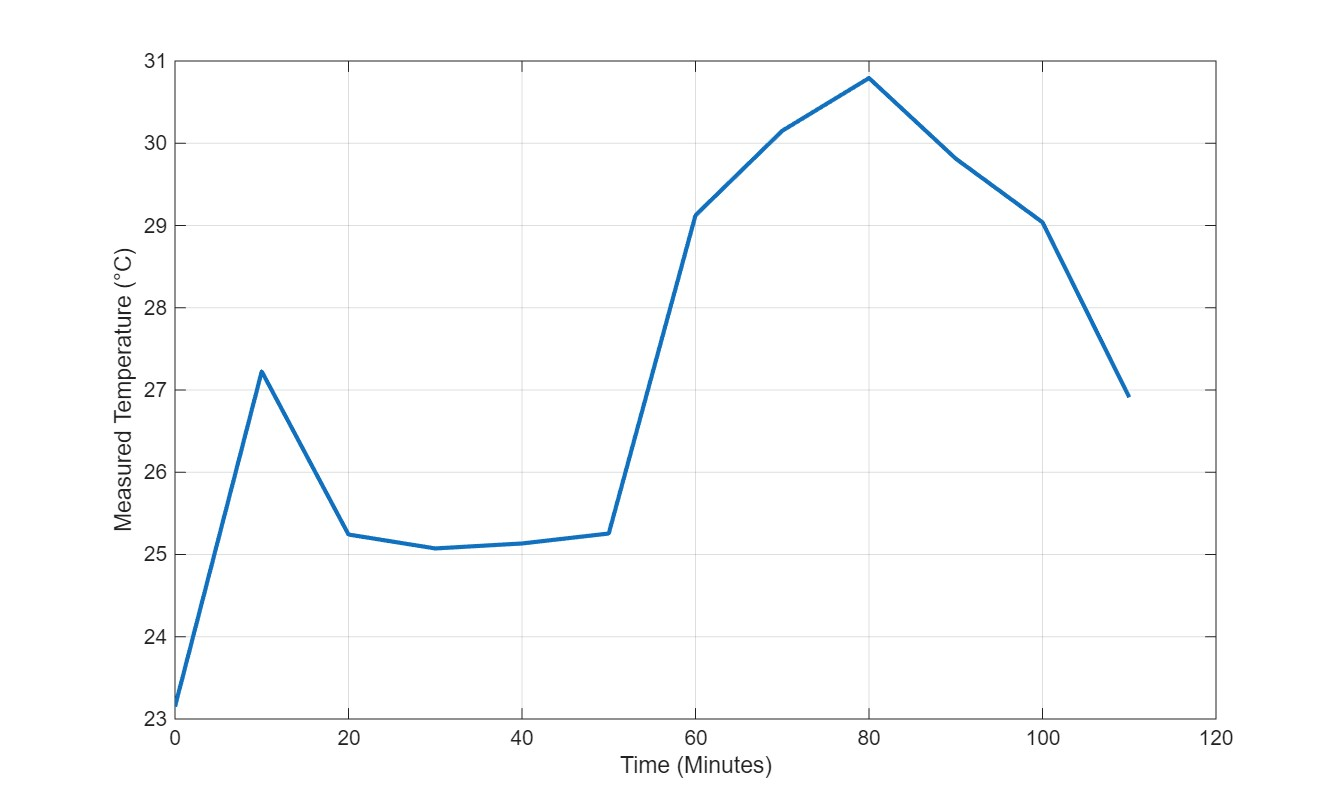
\includegraphics[width=\textwidth]{figs/Heat_Dissipation.jpg}
    \caption{Measured temperature vs time graph}
    \label{fig:Temperature}
\end{figure}


\section{Functionality Test}

The functionality tests are the tests required to be performed to determine whether the developed product functions as a medical-grade laparoscope. These are tests that require a testing station or a physical box trainer. These tests will be performed when the product is built and will illustrate if the product functions as desired.